
%%%%%%%%%%%%%%%%%%%%%%% file typeinst.tex %%%%%%%%%%%%%%%%%%%%%%%%%
%
% This is the LaTeX source for the instructions to authors using
% the LaTeX document class 'llncs.cls' for contributions to
% the Lecture Notes in Computer Sciences series.
% http://www.springer.com/lncs       Springer Heidelberg 2006/05/04
%
% It may be used as a template for your own input - copy it
% to a new file with a new name and use it as the basis
% for your article.
%
% NB: the document class 'llncs' has its own and detailed documentation, see
% ftp://ftp.springer.de/data/pubftp/pub/tex/latex/llncs/latex2e/llncsdoc.pdf
%
%%%%%%%%%%%%%%%%%%%%%%%%%%%%%%%%%%%%%%%%%%%%%%%%%%%%%%%%%%%%%%%%%%%


\documentclass[runningheads,a4paper]{llncs}

\usepackage{amssymb}
\setcounter{tocdepth}{3}
\usepackage{graphicx}

\usepackage{url}
\urldef{\mailsa}\path|{florian.hanika, gerhard.wohlgenannt|
\urldef{\mailsb}\path|marta.sabou|
\urldef{\mailsc}\path|erika.siebert-cole, peter.strasser, lncs}@springer.com|    
\newcommand{\keywords}[1]{\par\addvspace\baselineskip
\noindent\keywordname\enspace\ignorespaces#1}

\begin{document}

\mainmatter  % start of an individual contribution

% first the title is needed
\title{Crowdsourcing Enabled Ontology Engineering}
%Alternatives
%* Crowd-based ontology engineering
%* Tool support for crowd-based ontology engineering

% a short form should be given in case it is too long for the running head
\titlerunning{Crowdsourcing Enabled Ontology Engineering}

% the name(s) of the author(s) follow(s) next
%
% NB: Chinese authors should write their first names(s) in front of
% their surnames. This ensures that the names appear correctly in
% the running heads and the author index.
%
\author{Florian Hanika
\and Gerhard Wohlgennant
\and Marta Sabou}
\author{} % for initial submission
%
\authorrunning{Hanika et al.}
% (feature abused for this document to repeat the title also on left hand pages)

% the affiliations are given next; don't give your e-mail address
% unless you accept that it will be published

\institute{WU\
Vienna\\
\mailsa\\
\url{http://www.wu.ac.at}}

\institute{MODUL Univerisity\
Vienna\\
\mailsb\\
\url{http://www.wu.ac.at}}

\institute{}

%
% NB: a more complex sample for affiliations and the mapping to the
% corresponding authors can be found in the file "llncs.dem"
% (search for the string "\mainmatter" where a contribution starts).
% "llncs.dem" accompanies the document class "llncs.cls".
%

%\toctitle{Lecture Notes in Computer Science}
%\tocauthor{Authors' Instructions}
\maketitle


\begin{abstract}
Recent years have seen an increase in the use of crowdsourcing based methods at various stages of the ontology engineering lifecycle (e.g., verification of subsumption, assigning equivalences between concepts etc) thus laying the foundations of a novel approach to ontology engineering. Take up of this early research by the community at large, especially by practitioners, is however currently hampered by 1) a lack of understanding of which stages of the ontology engineering process can be crowdsourced and 2) tool support in ontology engineering platforms that would allow easy insertion of crowdsourcing into ontology engineering workflows. In this paper we perform an overview of recent works in the area and take a scenario-based approach to identifying those stages of the OE process where crowdsourcing makes sense. Then, we present the �uComp Protege plugin�, a plugin for the popular Protege ontology engineering platform that facilitates the integration of crowdsourcing stages into the OE process. TBD: clarify novelty (e.g., which new tasks we introduce?), sum up some important evaluation results.
\keywords{human computation, crowdsourcing, ontology engineering, ontology learning, Protege plugin}
\end{abstract}


\section{Introduction}

RQ1: Which tasks can be crowdsourced? How do they fit in the OE workflow?

RQ2: How to provide tool support for crowdsourcing in OE?



\section{Related Work - MS}

\subsection{Tools for Crowdsourcing}

The GATE Crowdsourcing Plugin is a first example of a plugin in a popular toolkit that allows crowdsourcing from within the tool.~\cite{Bontcheva2014}

\subsection{Use of Crowdsourcing for Knowledge Acquisition}

Siorpaes~\cite{Siorpaes2008} sees the use of games in supporting 3 major stages of the SW life-cycle:
\begin{enumerate}
\item Build and maintain SW vocabularies
\item Align SW vocabularies
\item Annotate content and maintain annotations
\end{enumerate}


Noy and colleagues~\cite{Noy2013} focus on the task of verifying subclass-superclass relations that make up the ontology hierarchy. Their main interest is in understanding whether crowdsourcing via MTurk is a viable alternative for this task and therefore they perform a series of experiments that compare microworkers against students, evaluate performance differences over different types of ontologies (e.g., upper ontologies vs. generic ontologies) and finally assess crowd-performance in specialized domains. The paper concludes that micro-workers are a viable alternative for verifying subclass-superclass relations and also introduces a vision for a tool support that would facilitate the integration of crowdsourcing into OE workflows. We present such a tool in this paper, that not only allows the ontology engineer to crowdsource subsumption verification, but also a set of other tasks that often appear in ontology engineering scenarios.

%Eckert - end goal: construction of hierarchies by aggregating human expert feedback on the relatedness and relative generality of terms; domain philosophy; Similar to us: "automatic OL methods are often weak on the task of determining the type of relation that holds between two terms" - I do not understand all details here ...

Eckert and colleagues~\cite{Eckert2010} relied on MTurk micro-workers to judge the relatedness of concept pairs (5-points scale between unrelated and related), as well as to specify the level of generality between two terms (more/less specific than). 

The CrowdMap system enlists micro-workers to solve the overall ontology alignment task~\cite{Sarasua2012}. It relies on two types of atomic HITS: the first one, asks crowdworkers to verify whether a given relation is correct ("Is conceptA the same As conceptB? yes/no "); the second task, requests micro-workers to specify how two given terms are related, in particular by choosing between sameAs, isAKindOf and notRelated. CrowdMap is designed to allow sameAs, subsumption or generic mappings between classes, properties and axioms, but currently it only support equivalence and subsumption mappings between classes.

%OntoPronto - decide whether a term is a class or an instance; then they relate this class to the most specific relevant PROTON class, therefore extending PROTON
The OntoPronto game~\cite{Siorpaes2008} is an example of game used for the creation and extension of Semantic Web vocabularies. Players are presented with a Wikipedia page of an entity and they have to firs judge whether this entity denotes a concept or an instance; and then relate it to the most specific concept of the PROTON ontology, therefore extending PROTON with new classes and instances. 

SpotTheLink  focuses on aligning Semantic Web vocabularies and has been instantiated to align the eCl@ss and UNSWPC~\cite{Siorpaes2008}  as well as  the DBPedia and PROTON ontologies~\cite{Thaler2011a}. The final version of the game, solves ontology alignment through two atomic tasks (1) choosing a related concept: given a DBPedia concept they need to choose and agree upon a related PROTON concept; (2) specifying the type of relation between two concepts in terms of equivalence or subsumption.

ZenCrowd~\cite{Demartini2012} focuses on the entity linking problem, where crowd-workers are used to verify the output of automatic entity linking algorithms. Concretely, given a named entity, e.g., "Berlin", and a set of dbpedia URLs generated automatically, crowd-workers have to choose all the URLs that represent that entity or "None of the above" if no URL is suitable. In essence this is an annotation task.

Guess What?!~\cite{Markotschi2010} creates ontologies by exploring instance data available as linked open data. Given a seed concept (e.g., banana), the game engine collects relevant instances from DBpedia, Freebase and OpenCyc and extracts the main features of the concept (e.g., fruit, yellowish) which are then verified through the collective process of game playing.The tasks performed by players are: (1) assigning a class name to a complex class description and (2) verifying previously generated class definitions.

[TBD: not sure about these - I think these refer to maintaining annotations]WhoKnows?~\cite{Waitelonis2011} and RISQ!~\cite{Wolf2011} have a similar mechanism: they use LOD facts to generate questions and use the answers to (1) evaluate property ranking (which property of an instance is the most important/relevant); (2) detect inconsistencies; (3) find doubtful facts. The obtained property rankings reflect the �wisdom of the crowd� and are an alternative to semantic rankings generated algorithmically based on statistical and linguistic techniques. The games differ in the gaming paradigm they adopt. While WhoKnows?! uses a classroom paradigm and aims towards being an educational game, RISQ! is a Jeopardy-style quiz game. 

Climate Quiz~\cite{Scharl2012a} is a Facebook game where players evaluate whether two concepts presented by the system are related (e.g. �environmental activism�, �activism�), and which label is the most appropriate to describe this relation (e.g. �is a sub-category of�). The possible relations set contains both generic (�is a sub-category of�, �is identical to�, �is the opposite of�) and domain-specific (�opposes�, �supports�, �threatens�, �influences�, �works on/with�) relations. Two further relations, �other� and �is not related to� were added for cases not covered by the previous eight relations. The game�s interface allows players to switch the position of the two concepts or to skip ambiguous pairs.

\begin{table}
%\footnotesize

\center
\begin{tabular}{|l|l|c|c|} \hline
\textbf{Approach}&\textbf{Solved Task}&\textbf{Example}& \textbf{HC Genre}\\ \hline

InPho~\cite{Eckert2010} & specification of subsumption relations & Dualism moreSpecificThan Philisophy of mind& MLab\\ \hline
					& term relatedness judgemendts & epistemology vs. virtue epistemology & MLab\\ \hline
CrowdMap~\cite{Sarasua2012} & Verification of subsumption/eqv relations & Is conceptA the same As conceptB? & MLab\\ \hline
			& Specification of subsumption/eqv relations &  & \\ \hline
~\cite{Noy2013} & Verification of subsumption relations & TBD& MLab\\ \hline
OntoPronto~\cite{Siorpaes2008} & Class vs. instance decisions & & GWAP\\ \hline
 & Creation of SubClassOf/InstanceOf relations & &\\ \hline
SpotTheLink~\cite{Thaler2011a} & Choosing a related concept & Is FilmFestival relate to Happening, Abstract or Object? & GWAP\\ \hline
 & Creation of eqv/subsupmtion relation & Is FilmFestival equivalent/more specific than Happening?&\\ \hline
ZenCrowd~\cite{Demartini2012} & text to URL mapping (annotation) & &\\ \hline
Guess What?!~\cite{Markotschi2010}& verify complex class definitions  & Banana: fruit \& yellow \& grows on trees&\\ \hline
& generate class names for complex defs  & &\\ \hline
Climate Quiz~\cite{Scharl2012a}  & specify relations between terms  & &\\ \hline


\end{tabular}
\caption{Overview of ontology engineering tasks typically solved with crowdsourcing.}
  \label{table:tasksFromRW}
  \end{table}
  
  

\section{Ontology Engineering Scenarios - Ontology Learning - MS}
 (1 or both of the following)
OL - Gerhard�s work on automatic OL from text \& other sources

OR - using the Watson plugin

TBD: Relate to the "Embedded HC paradigm" => other approaches that enhance algorithms are CrowdMap and ZenCrowd

\section{Ontology Engineering Tasks for Crowdsourcing - MS}

From the scenarios above as well as the related work, we distinguish a set of generic ontology engineering tasks that are suitable for crowdsourcing and which are likely to be of interest in a wide range of ontology engineering scenarios:

\begin{description}
\item[T1. Verification of Domain Relevance.]  Is a concept/instance relevant for a domain? 
\item[T2. Verification of Relation Correctness.] Does a certain relation between two ontology entities hold? These could be a set of generic relations (sameAs, subClassOf, instanceOf), but also arbitrary named relations to be specified by the ontology engineer. The crowd here would have to vote (yes/no) for a given triple (Subject - Relation - Object). This task is the focus of [1].
\item[T3. Learning of Relation Names.] This is also a very difficult task in OL in general - the workers are presented with two terms and can choose between a set of given relations what applies. These relations can be a set of OWL relations that all ontologies have as well as a (restricted) number of domain specific relations specified by the expert (e.g., �influences�). [BTW, since this is a complex task it could be split up into a sequence of 3 simpler tasks: 1) given two terms workers agree whether these are related or not; 2) those pairs that were judged related are then passed to another task where a correct relation is selected; 3) in the third task, the quality of the relations is checked - practically T2]
Available relation labels are some predefined (like subClassOf) and those from the target ontology (all ObjectProperties) -- if more than 20 .. spread over multiple windows (depending on window size)
Have a limit of 5 relation labels in the Protege interface
All pairs with a certain relation (defined by the user in a text field, eg �relation�) are sent to the uComp API (or directly to CF).
If you want to use just a subset of relations: have a window where you select (checkboxes) the actual pair to be sent.
In CrowdFlower -- also have the choice to add a free text label
output: be able to sort by certainty from CF ..
\end{description}

\section{The uComp Protege Plugin - GW}
This section describes the actual plugin, ie.~which tasks have been implemented, and the features and usage of the plugin.
Protege was developed in Java, it can easily be extended in the form of \emph{plugins} which are typically Java Archive (.jar) files
stored in the Protege \texttt{plugin} directory. The most common form of a Protege plugin is a \emph{view plugin}, which implements a single view for a specific area of an ontology (e.g. classes, individuals, object properties, \dots).
%Florian: Protege completely was programmed in Java, therefore all plugins also are programmed in Java. Since Protege was developed very modular, it is quite easy to create simply plugins and integrate them into Protege. 
%Florian: All Protege plugins are so called jar-Files (Java Archive), and contains the compiled source code and all needed libraries. The most common form of a Protege plugin is a view plugin, which implements a single view for a specific area of an ontology (e.g. classes, individuals, object properties, ...)

% installation / SETUP 
\textbf{Installation and setup.}
The plugin is available at \url{TODO -- add link once uploaded to Protege}, includes detailed documentation about the tasks and
the usage of the plugin. TODO (if necessary) documentation is accessible at ..
To use the plugin you need to your uComp-API key\footnote{Request a key from the uComp team, see \url{http://soc.ecoresearch.net/facebook/election2008/ucomp-quiz-beta/api/v1/documentation/}} in a file named \texttt{ucomp\_api\_key.txt} in folder \texttt{.Protege}.


%Florian: The CF key has to be associated with the uComp-API key, therefore it has to be communicated to the uComp-API team (see http://soc.ecoresearch.net/facebook/election2008/ucomp-quiz-beta/api/v1/documentation/)
%Florian: The uComp-API key itself must be put into a textfile named "ucomp_api_key.txt" at the users home directory, in the folder ".Protege" (which is created by Protege during installation on both Windows and Linux plattforms) 

%Florian: all information about the task is stored (depends on the kind of task): domain, validation of whole subtree going on?, additional information, sent to crowdflower or ucomp-quiz, ucomp-api job-id, ...

% give an example SCREEENSHOT with a quick introduction 
\begin{figure*}[htb]
\centering
{\centering \resizebox*{1.0\textwidth}{!}{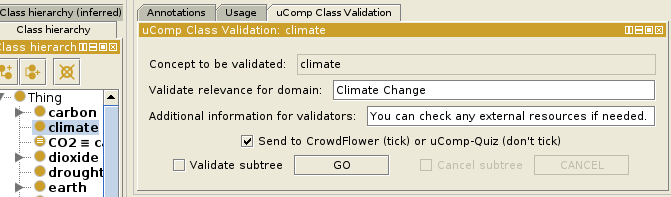
\includegraphics{images/c_rel_check_start.png}}}
 \caption{\label{fig:screen_cr}Screenshot showing the interface for validating a concept.}
\end{figure*}

Figure~\ref{fig:screen_cr} shows the basic interface for the domain relevance task, the other tasks
have similar interface.
Initially, the user adds the new view in the Protege window. The plugin interface contains
task specific information (eg. the concept selected by the user for validation),
generic information such as the \emph{domain} of the ontology and \emph{additional information} (see below),
and a \texttt{GO} button start the validation process. \\


% The common PROCESS (in short)
\textbf{Usage.} The process itself is similar for all types of evaluations:
\begin{enumerate}
\item Add the corresponding view to the user interface via the \emph{Window $\rightarrow{}$ Views} menu. The ontology engineer
selects the part of the ontology to verify (eg. the \emph{classes}), and adds the corresponding uComp HC validation frame to the user interface. 
\item The user selects which part of the ontology should be verified (eg. a specific class or all classes in the ontology).
\item The user can provide additional information and options in the plugin view and then starts the evaluation.
\item A requested is sent to the uComp API.
\item Depending on user settings, the uComp API delegates the job to a GWAP or to CrowdFlower.
\item As soon as available, the plugin presents the results to the user and saves them in the ontology.
\item The user can always cancel (pause) the validation process.
\item Depending on the result, the user will perform further actions such as deleting parts of the ontology which have been validated as non-relevant.
\end{enumerate}

%After enough HC users given their input on the task, the results are sent back to the plugin, which then displays them to the Protégé user. 
%Depending on the result, the user can perform further actions like deleting negatively validated parts of the ontology.


% PERSISTENCE 
All data collected by the plugin which should be persistent is stored in the ontology in \texttt{rdfs:comment} fields,
for example information about the domain, the job ID, and results from the game.


% COMMON FIELDS in the UI: domain and additional information & validate subtree
\textbf{The User Interface}
What is common among all tasks handled by the plugin, is the selection of a \emph{domain} and that the user can provide
additional information about the task. The domain is simply the field of knowledge which the ontology covers. If entered
once, the domain will be stored in the ontology (as \texttt{rdfs:comment}) and be pre-filled subsequently, but it can also be changed at any time.
For every task, the plugin contains a predefined task description (typically including examples) which is presented to the HC user.
If the ontology engineer wants to extend this task description, he or she can provide more guidelines in the field \emph{additional information}.
In many cases the user of the plugin wants to verify not only a single class, but a part of the ontology, or even the whole ontology.
This can be achieved with the \emph{Validate subtree} option. If the option is selected, the current concept and all its subconcepts 
are verified (recursively). The verify the entire ontology, the user just starts from the uppermost class (\emph{Thing}).
In the remainder of the section we give some details about the parts of the plugin used in the evaluation (see Section~\ref{sec:eval}),
ie.~verification of domain relevance and of relation correctness.
%Florian: domain will be stored as rdfs:comment in the head of the ontology

% T1. Verification of Domain Relevance.  Is a concept/instance relevant for a domain?
% T2. Verification of Relation Correctness. Does a certain relation between two ontology entities hold? These could be a set of generic relations (sameAs, subClassOf, instanceOf), but also arbitrary named relations to be specified by the ontology engineer. The crowd here would have to vote (yes/no) for a given triple (Subject - Relation - Object). This task is the focus of [1].


% TASKs
\textbf{Task 1 - Verification of Domain Relevance.}
Verification of domain relevance of a class (called ``uComp Class Validation'' in the plugin) helps to decide if a concept (class) is relevant for a domain. 
First, the ontology engineer adds the corresponding view (\emph{Window} $\rightarrow{}$ \emph{Views} $\rightarrow{}$ \emph{Class Views} $\rightarrow{}$ \emph{uComp Class Validation}) to the UI.
This is the simplest type of validation task, so the process is very much in line with the \emph{usage} described above.
Figure~\ref{fig:screen_cr} shows the UI for the class ``fracking'' before initiating the verification. 

\begin{figure*}[htb]
\centering
{\centering \resizebox*{1.00\textwidth}{!}{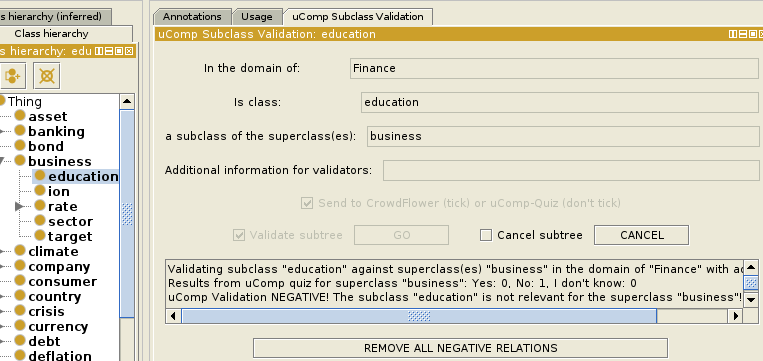
\includegraphics{images/sc_subclass_val.png}}}
 \caption{\label{fig:screen_sub}Screenshot showing the interface for subClassOf relation validation, including the display of results}.
\end{figure*}


\textbf{Task 2 - Verification of Relation Correctness.}
The second task is the verification of relation correctness, more precisely the verfication of IS-A (subClassOf) relations between classes.
The corresponding view is named \emph{Class Views} $\rightarrow{}$ \emph{uComp SubClass Validation}. When selecting a class in Protege,
the plugin automatically detects its superclasses (if any) and fills the boxes in the plugin UI.
As soon as results are available these are presented in the UI, as shown in Figure~\ref{fig:screen_sub}. The screenshot gives an example
wit one evaluator, who rated the \emph{IS-A} relation between ``education'' and ``business'' as invalid. As the majority of ratings is negative,
a button to remove the relation is displayed.

\textbf{Task 3 - 5.}
The uComp Protege plugin also supports 3 other tasks, which we will cover only briefly, as they are not part of the user evaluation in
Section~\ref{sec:eval}. Task 3 is the verfication of \emph{instanceOf} relations between an individual and a class, i.e.~the crowd helps
to verify if a given \emph{instanceOf} is valid. Task 4 is concerned with validating \emph{domain} and \emph{range} of properties, which
results in two separate sub-tasks (domain, range). And finally, we implemented a Protege view component that collects suggestions for 
labelling unlabeled relations from a set of given properties (relations).


\section{Evaluation}
\label{sec:eval}

\subsection{Evaluation Goal}
The goal of the evaluation is to assess the improvements that the uComp Plugin could enable in a typical ontology engineering scenario in terms of typical project completion aspects such as time, cost and quality of output. The usability of the plugin is an additional criteria that should be evaluated. Concretely, our evaluation goals can be summarised into the following questions:

\begin{description}
\item[Time] \textit{How does the use of the plugin affect the time needed to perform ontology engineering tasks?} - We distinguish here the total task time (Ttt) as the time taken from the start of the ontology engineering task until its finalisation; and the time of the ontology engineer spent actively in the task (Toe). In a crowdsourced scenario, Toe < Ttt, because the ontology engineer is only actively working during the outsourcing of the task and the review of the result. In contrast, in a traditional scenario Toe = Ttt. What is of interest to us is the time reduction ratio, that is (Ttt-Toe)/Ttt. (this will be computed as an average over multiple measurements, and over various ontology engineering tasks).

\item[Cost] \textit{Are there cost benefits associated with the use of the plugin?}  We compute costs related to payments for the involved work-force, that is payments to ontology experts and payments to crowd-workers. Costs of ontology experts are computed by multiplying the time they spend on the task (Toe) with an average salary. In order to allow comparison to other similar cost-focused studies [1], the wage of a research scientist was assumed to be \$54,000 per annum.

\item[Quaility] \textit{What are the implications on the quality of the resulting output when using the Plugin?} Several earlier studies [e.g., Thalhammer�13, Sabou�13, Noy?, Sabou�13] have shown that the quality of the semantic tasks performed by crowd-workers is in general similar to (or even better than) the quality of tasks performed by ontology engineers. While the quality of the obtained data is not the core focus of our evaluation, we expect to obtain results similar to those already published [TBD: note however, that unlike earlier studies which focus on simple, atomic tasks, we focus on more complex engineering tasks - is this really true?]

\item[Usability] \textit{Is the plugin usable?} As any end-user tools, the plugin should be easy to understand and use by the average ontology engineer already familiar with the Protege environment.
\end{description}

\subsection{Evaluation Setup}

The setup involves working with two groups of ontology engineers, which will perform the same OE  tasks. 

\subsubsection{Evaluators}

Victims: Adrian, J�rgen (? knows the tool), 2 guys from TU Vienna (Olger, Fajar)
Non-Protege victims: Stefan, Matyas, Michael, Philipp, Heinz, Max G�bel

\begin{description}
\item[Group 1]  This group will make use of traditional (that is manual) methods to perform the three OE tasks. The group consists of X ontology engineers.
\item[Group 2] This group, consisting of Y ontology engineers,  will use the Plugin to perform the three OE tasks. Group 2 will be provided a short tutorial about the plugin (30 minutes) and will have to perform a usability questionnaire about the plugin.
\end{description}

\subsubsection{Evaluation Data}
The input to all evaluation tasks are ontologies generated by an ontology learning algorithm from textual sources. 

For every ontology snapshot, ie. every result of an ontology learning stage, as well as the resulting ontology the system exports an OWL file (using the Turtle seralization format, which can be converted to RDF/XML easily).
The conversion of our internal format for lightweight ontologies is straightforward for concepts (which resemble to OWL classes). WordNet hyper- and hyponym relations are mapped to the OWL subClassOf property. The only challenging aspect is the representation of unlabeled relations in OWL. Our system creates ObjectProperties named "relation\_n", where "n" is an auto-incrementing number, as it is not possible to use the same ObjectProperty more than once. The label for those relations is plainly "relation". The periodically created versions of the domain ontology can be uploaded to a triple store and are thereby accessible via the SPARQL.

We evaluate the plugin over two ontologies covering two diverse domains. Some details of the input ontologies are:

\begin{table}
%\footnotesize

\center
\begin{tabular}{|l|l|c|} \hline
&\textbf{Climate Change Ontology}&\textbf{Finance Ontology}\\ \hline


\textbf{Nr. of Classes} & 101  & 77 \\ \hline
\textbf{Nr. of Relations} & 62  & 50  \\ \hline
\textbf{Nr. of IsA Relations} & 43  & 20  \\ \hline
\textbf{Nr. of Un-named Relations} & 18  & 30 \\ \hline

\end{tabular}
\caption{Overview of the ontologies used in the experiments.}
  \label{table:surveygwaps}
  \end{table}


\subsubsection{Evaluation Tasks}
We perform the evaluation of the plugin over three different ontology engineering tasks in order to 1) test different functionalities of the plugin; 2) obtain evaluation result over a range of tasks.

Both user groups will perform the following tasks:

\begin{description}
\item[Task 1: Check concept relevance for a domain] For each concept of the ontology decide whether it is relevant for the domain in question (in our case, climate change). Input: concept and domain name; Output: Y/N ratings -- use a relevant\_to\_domain property -- domain experts use �Y/N�

\item[Task 2: Check the correctness of isA relations] For all isA relations verify whether they are correct, that is a generic/specific relation exists between the domain and range of the relation. Manual experts change the value for a certain annotation property (...\_subClass\_validation\_result)
\end{description}

\subsubsection{Evaluation Metrics}

For time:
For each participant measure Toe, and Ttt, for each task.
Compute averages per participant
Compute group averages and differences
 
For costs:
Compute avg costs per participant and per group and differences
 
For quality: Since we do not have a baseline, we will proceed as follows:
Task 1: compute pair-wise inter-expert agreement for both groups; and between groups � this will measure how different the output is between the plugin and non-plugin group. If it is small then the results are similar; Compute also Cohen�s Kappa
Task 2: same approach as with Task 1
Task 3: Here I think we should evaluate the quality of labels ourselves (em and Gerhard) for each produced ontology; and then  compute a precision value

\bibliographystyle{plain}
\bibliography{cl-iswc14}


\end{document}
